% -- NAO MUDAR O TAMANHO DA FONTE.
% -- O USO DO TAMANHO DA FONTE EM 12PT Eh OBRIGATORIO
\documentclass[12pt]{article}

% -- O USO DO TEMPLATE DA SBC Eh OBRIGATORIO
% -- NAO ALTERAR NENHUMA PARAMETRO DO MODELO DA SBC
% -- (E.G., MARGENS LATERAIS, RODAPE, CABECA�HO, ENTRE OUTROS)
\usepackage{sbc-template}

\usepackage{graphicx,url}

%\usepackage[brazil]{babel}
\usepackage[latin1]{inputenc}

% descomente abaixo caso tenha problemas com a numera��o das se��es n�o
% aparecerem. Em especial no Ububtu 16.x
%\usepackage{etoolbox}
%\makeatletter
%\patchcmd{\ttlh@hang}{\parindent\z@}{\parindent\z@\leavevmode}{}{}
%\patchcmd{\ttlh@hang}{\noindent}{}{}{}
%\makeatother

%macros
\newcommand{\tit}[1]{\textit{#1}}
\newcommand{\tbf}[1]{\textbf{#1}}
\newcommand{\ttt}[1]{\texttt{#1}}

% -- O USO DESTE COMANDO Eh OBRIGATORIO
\sloppy

% -- CERTIFIQUE-SE DE QUE O TITULO NAO ESTEJA ULTRAPASSANDO OS LIMITES
% -- DAS MARGENS.
% -- USE O COMANDO QUEBRA-DE-LINHA (\\) SE TITULO FOR MUITO LONGO.
\title{Visual Attention with Deep Learning}

% -- CERTIFIQUE-SE DE QUE O NOME DOS AUTORES ESTEJA CORRETO.
% -- EM GERAL COLOCA-SE O ALUNO COMO PRIMEIRO AUTOR E O ORIENTADOR COMO
% -- ULTIMO AUTOR.
\author{Erik Perillo\inst{1}, Esther Luna Colombini\inst{1}}

% -- CERTIFIQUE-SE DE QUE OS NOMES DAS INSTITUICOES E SEUS RESPECTIVOS ENDERECOS
% -- NAO ESTEJAM ULTRAPASSANDO OS LIMITES DAS MARGENS. SE ISTO OCORRER, USE O
% -- COMANDO QUEBRA-DE-LINHA (\\) OU ABREVIACOES APROPRIADAS.
\address{Institute of Computing (IC) -- University of Campinas
  (Unicamp)\\
  Caixa Postal 6176 -- 13.084-971 -- Campinas -- SP -- Brazil
  \email{erik.perillo@gmail.com, esther@ic.unicamp.br}
}


% -- CERTIFIQUE-SE DE QUE AS TABELAS E FIGURAS INSERIDAS NO
% -- DOCUMENTO NAO ESTEJAM ULTRAPASSANDO
% -- OS LIMITES DAS MARGENS.

\begin{document}

\maketitle

% -- O RESUMO EM INGLES Eh OBRIGATORIO,
% -- INDEPENDENTE DO IDIOMA EM QUE TRABALHO FOI ESCRITO
\begin{abstract}
Vision is a key element in one's process of understanding the world.
The high volume of sensorial data is however problematic because
most of the information is often irrelevant.
Humans realize sensorial filtering by what we call attention.
We propose the application of Deep Learning for obtaining a visual salience
system which behaves similarly to humans.
We built a new convolutional neural network with relatively
simple architecture, yielding a performance level consistently among the
best ten state of the art models in MIT300 benchmark.
\end{abstract}

% -- O RESUMO EM PORTUGUES Eh OBRIGATORIO, INDEPENDENTE DO
% -- INDIOMA EM QUE O TRABALHO FOI ESCRITO
\begin{resumo}
A vis�o � elemento-chave no processo de entender o mundo para um ser.
Entretanto, a alta quantidade de dados sensoriais � problem�tica,
havendo muitas vezes irrelev�ncia de informa��o.
Nos seres humanos, h� um filtro sensorial realizado pela aten��o.
Propomos a aplica��o de
\tit{Deep Learning} para a obten��o de um sistema de sali�ncia visual que
se comporte como o dos seres humanos.
Constru�mos uma nova rede neural convolucional de arquitetura relativamente
simples e com um desempenho que a coloca consistentemente entre os dez
melhores modelos estado da arte no \tit{MIT300 benchmark}.
\end{resumo}

\section{Introduction}
One of the most challenging unsolved problems in Artificial Intelligence is
vision.
It is fundamental for the conception of systems that interact with the real,
physical world.
Such systems would be useful for applications that involve
robotics and tasks in domestic houses, industry and agriculture, so
there is great potential for the benefit of society.

Vision is remarkably data and computationally intensive:
In humans, approximately half the brain is involved in
vision-related tasks~\cite{fixott_1957}.
Even our brains can't handle all the sheer amount of sensorial information
that we receive every second: We have attention, a fundamental mechanism
that, among other functionalities, filters out irrelevant information
-- either visual or from other senses-- and helps us focus our cognitive
processes on what is important at a given moment.
These facts are a strong evidence that, in order to solve
vision, we need to have attention.

\subsection{What is visual saliency?}
Visual saliency can be defined as the delimitation of a certain spatial
region on an image for further cognitive processing~\cite{treisman_1980}.
Psychologists have been studying for at least half a century what makes we
direct our visual focus to a certain region and how we do it.

The phenomenon of visual saliency may emerge from two fundamentally
different processes:
There is \emph{top-down} attention, an internal
stimuli of the agent (e.g. find a red apple in a tree because of hunger,
which will automatically make red be reconizable more easily on the scene),
and \emph{bottom-up} attention, an external process which captures the
agent's attention from abrupt changes in visual stimuli or high contrast.
It has been shown that some patterns are naturally visually salient for humans.
Some of them are: color contrast (specially green-red and yellow-blue),
luminance contrast, orientation contrast, high
frequency movement~\cite{colombini_2016}.
In this work, we focus on \emph{bottom-up} attention.
\begin{figure}[hbt]
\begin{center}
		\begin{tabular} {cc}
		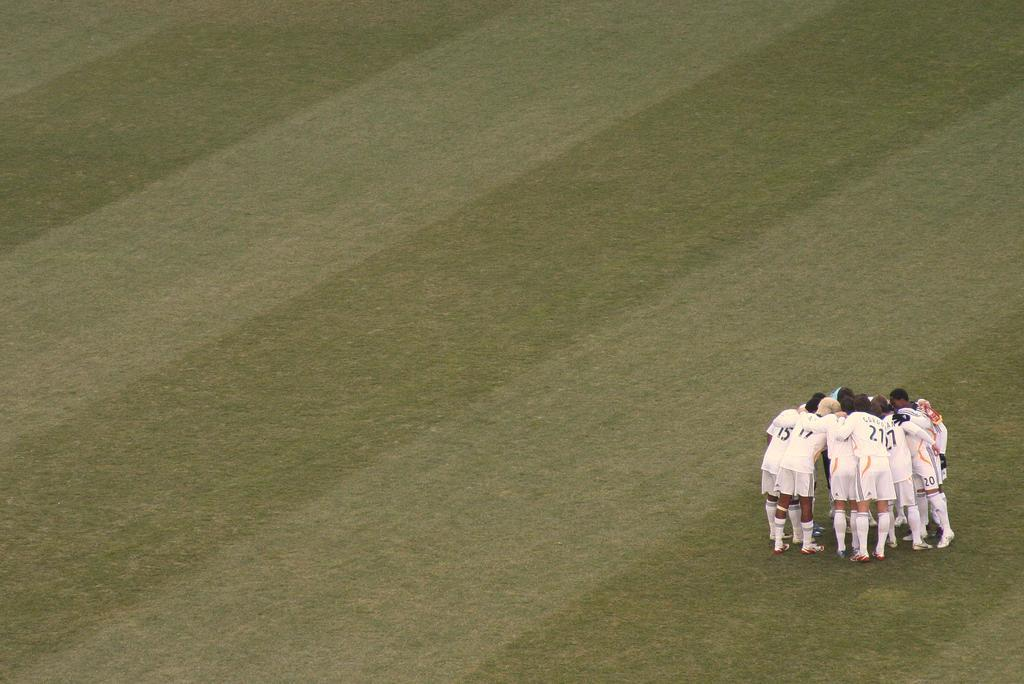
\includegraphics[width=0.5\textwidth]{./img/soccer_s.jpg} &
		
\includegraphics[width=0.5\textwidth]{./img/soccer_m.jpg}\\
        (a) & (b)
		\end{tabular}
\end{center}
\caption{Example of visual saliency.
    b) is the salience map where brighter pixels represent regions more
    salient to humans on the original image a).}
\label{fig:example}
\end{figure}

Visual salient regions on images are usually represented by
\emph{saliency maps}.
Such maps are grayscale images generated such that
areas with pixels close to white express high saliency
of the same region on the original image, whereas regions with pixels close
to black represent a region of low saliency.
Datasets with pairs image-map are usually obtained by colleting eye-fixation
data from humans that looked at the images.

\subsection{Related work}
Early computational models of visual saliency were generally built based on
filtering of images for extraction of a pre-selected set of features
considered important for \emph{bottom-up} attention.
Many of them are based on theoretical models of attention, such as the
\emph{Feature Integration Theory}~\cite{treisman_1980}
and \emph{Guided Search}~\cite{wolfe_1989}.
\emph{Vocus}~\cite{frintrop_2005} is a computational model that extracts
features such as color contrast, orientation and luminance contrast from
different scales of the image to produce saliency maps in the style of
figure~\ref{fig:example}b.

A rapid change of paradigm ocurred around 2015 when \emph{Deep Learning}
techniques showed to be extremely effective in the generation of saliency
maps.
Models such as \emph{Salicon}~\cite{jiang_2015} showed that applying
convolutional neural networks with weights initialized from networks used
for image classification, e.g. \emph{VGG-16}~\cite{zisserman_2014}
could yield maps very similar to those generated from humans.
Later works further explored this idea.
\emph{ML-net}~\cite{cornia_2016} uses the output from different layers
of \emph{VGG-16} to use information from various dimensions and levels of
abstraction.
\emph{DeepFix}~\cite{kruthiventi_2015} extends a pre-trained model with
new layers that account for global features and center bias.
\emph{Salnet}~\cite{pan_2016} is a work that explores two models that are
remarkably simple yet provides good results.
As of today, at least nine out of the ten best models in the ranking of the
\emph{MIT saliency benchmark}~\cite{mit_sal_bm} use \emph{Deep Learning}
techniques.

\subsection{Motivation}
Current state of the art models are in general quite expensive computationally,
partly because most of them are based on very big pre-trained networks.
Even \emph{Salnet}, one of the simplest models, is composed
of 25.8 million parameters.
While pre-trained weights from classification tasks showed to be effective
for saliency prediction, it is reasonable to question whether
creating a network from scratch could yield a smaller amount of parameters
that are more efficient for the sole task of salience prediction.
Also, there are some ideas from previous work on psychology that weren't
found to be used in current models but are considered worthwhile to be
explored.

\subsection{Objectives}
This work aims at building a visual saliency model that is a) effective,
yielding results similar to other state of the art models,
and b) relatively simple and computationally efficient.
It is important that both criteria are matched because we aim at extending the
model in the future for video and real time applications such as
navigating robots.
We build a novice fully convolutional neural network.
A previously built classical model, which is strongly based on \emph{Vocus},
is used for comparison purposes.

\section{Methodology}
\begin{itemize}
    \item Old method: be succint
    \item New method: architecture, datasets, datapreproc, training
\end{itemize}

\begin{figure}[hbt]
    \centering
    \def\svgwidth{\columnwidth}
    \input{./img/model.pdf_tex}
    \label{fig:model}
    \caption{Overview of the network architecture.
        Filters are in format width$\times$height\_stride.}
\end{figure}

\begin{figure}[hbt]
    \centering
    \def\svgwidth{0.7\linewidth}
    \input{./img/inception.pdf_tex}
   \label{fig:inception}
    \caption{Inception block layout.}
\end{figure}


\begin{table}[H]
\centering
\begin{tabular}{|c|c|c|}
	\hline
	Block number & Filter name & Number of filters\\
	\hline
    1 & conv 1 & 48\\
    \hline
    2 & conv 1 & 64\\
    \hline
    2 & conv 2 & 96\\
    \hline
    3 & conv 1 & 128\\
    \hline
    3 & conv 2 & 128\\
    \hline
    3 & conv 3 & 144\\
    \hline
    3 & conv 4 & 144\\
    \hline
\end{tabular}
\end{table}

\begin{table}[H]
\centering
\begin{tabular}{|c|c|c|c|c|c|c|}
	\hline
    Block number & conv 3x3 reduce & conv 3x3 & conv 5x5 reduce & conv 5x5
    & conv 1x1 & pool\\
    \hline
    1 & 32 & 64 & 24 & 48 & 64 & 64\\
    \hline
\end{tabular}
\end{table}


\section{Results}
\begin{itemize}
    \item Old method
    \item New method, mit300 bm
\end{itemize}
\section{Conclusion}
\begin{itemize}
    \item Ey, that's pretty good
    \item next steps
\end{itemize}

% -- NAO MUDAR O ESTILO DAS REFERENCIAS BIBLIOGRAFICAS. O USO DO PADRAO DA SBC Eh OBRIGATORIO
\bibliographystyle{sbc}
\bibliography{sbc-template}

\end{document}
